\documentclass[a4paper]{jarticle}
\usepackage{graphicx}
\begin{document}

定規でどう測っても幅 (縁含む) 40mm なのだけど、
そこのファミマの印刷機だと 42mm でぴったりだった.
印刷して出てきたのを測るとやっぱり 40mm だった.

\begin{figure}
  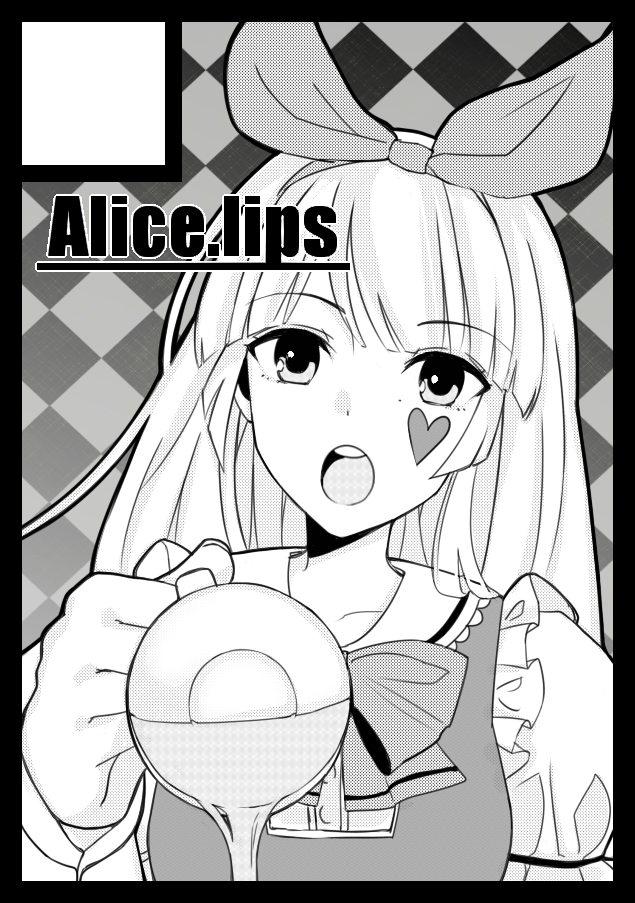
\includegraphics[width=40mm,bb=0 0 600 853]{AliceLips.png}
  \hfill
  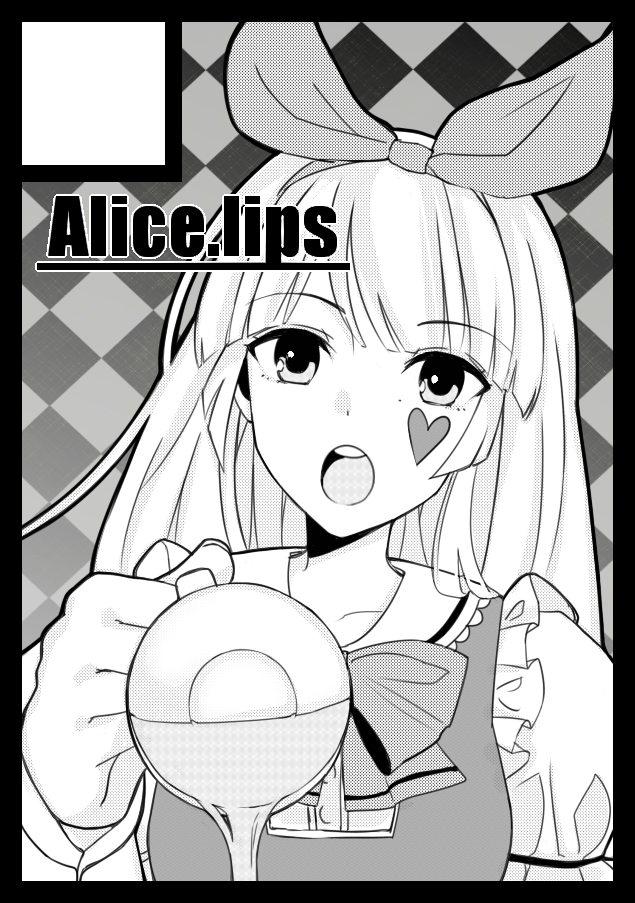
\includegraphics[width=40mm,bb=0 0 600 853]{AliceLips.png}
  \caption{width=40}
\end{figure}

\begin{figure}
  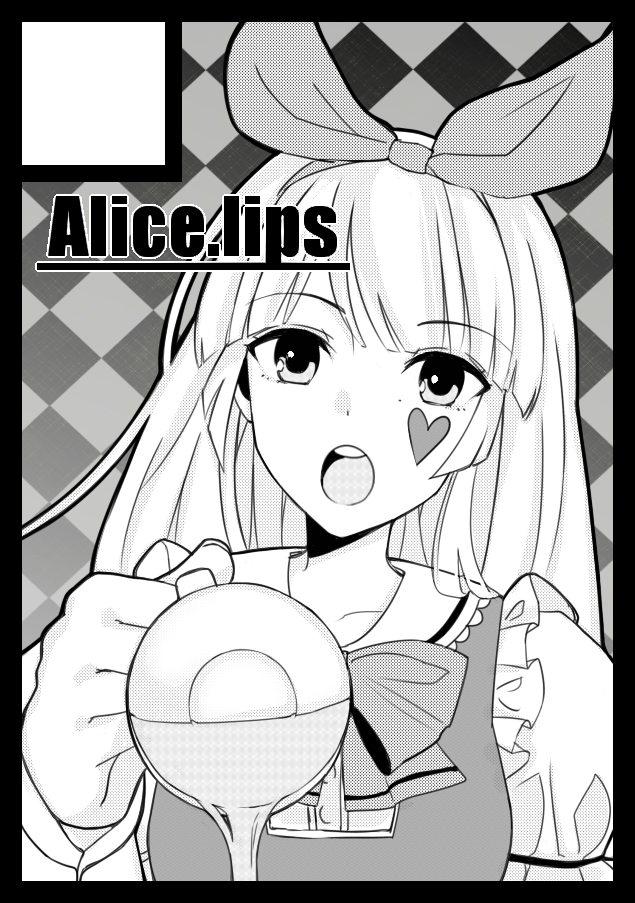
\includegraphics[width=42mm,bb=0 0 600 853]{AliceLips.png}
  \hfill
  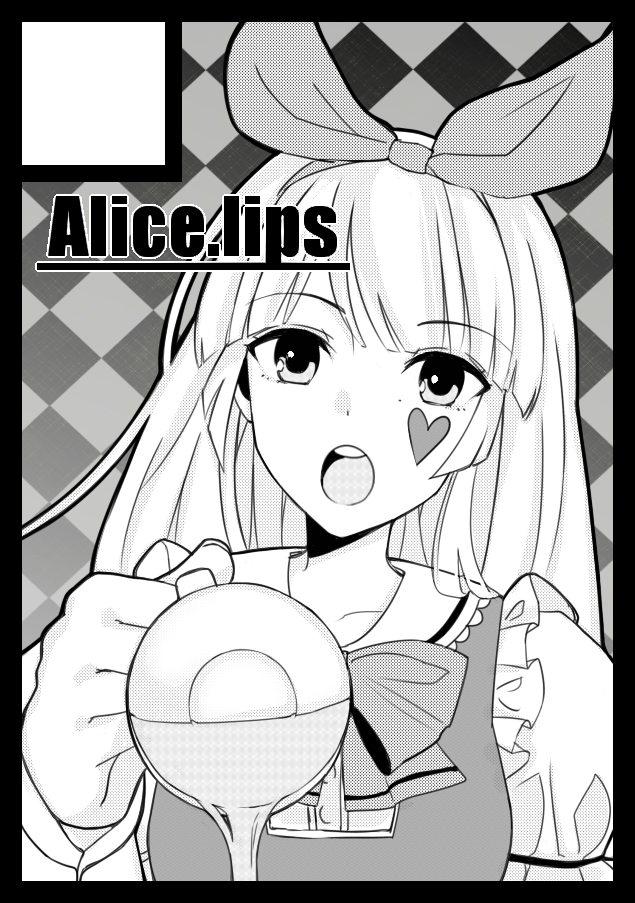
\includegraphics[width=42mm,bb=0 0 600 853]{AliceLips.png}
  \caption{width=42}
\end{figure}

\end{document}
